\newpage
\section{Methodology}
\label{sec:methodology}

\subsection{MAPPO Framework Overview}
\label{subsec:mappo-overview}

The proposed method follows the centralized training with decentralized execution (CTDE) paradigm. During training, a centralized critic observes the global simulator state and provides a learning signal that captures system-wide congestion, load balance, and PRB usage. During execution, each device acts independently based only on its own local observation and the feasible-destination mask. This separation is well suited to the target edge-computing scenario because global state is available during simulation and offline training, but real-time deployment should avoid a centralized bottleneck.

\begin{figure}[htbp]
    \centering
    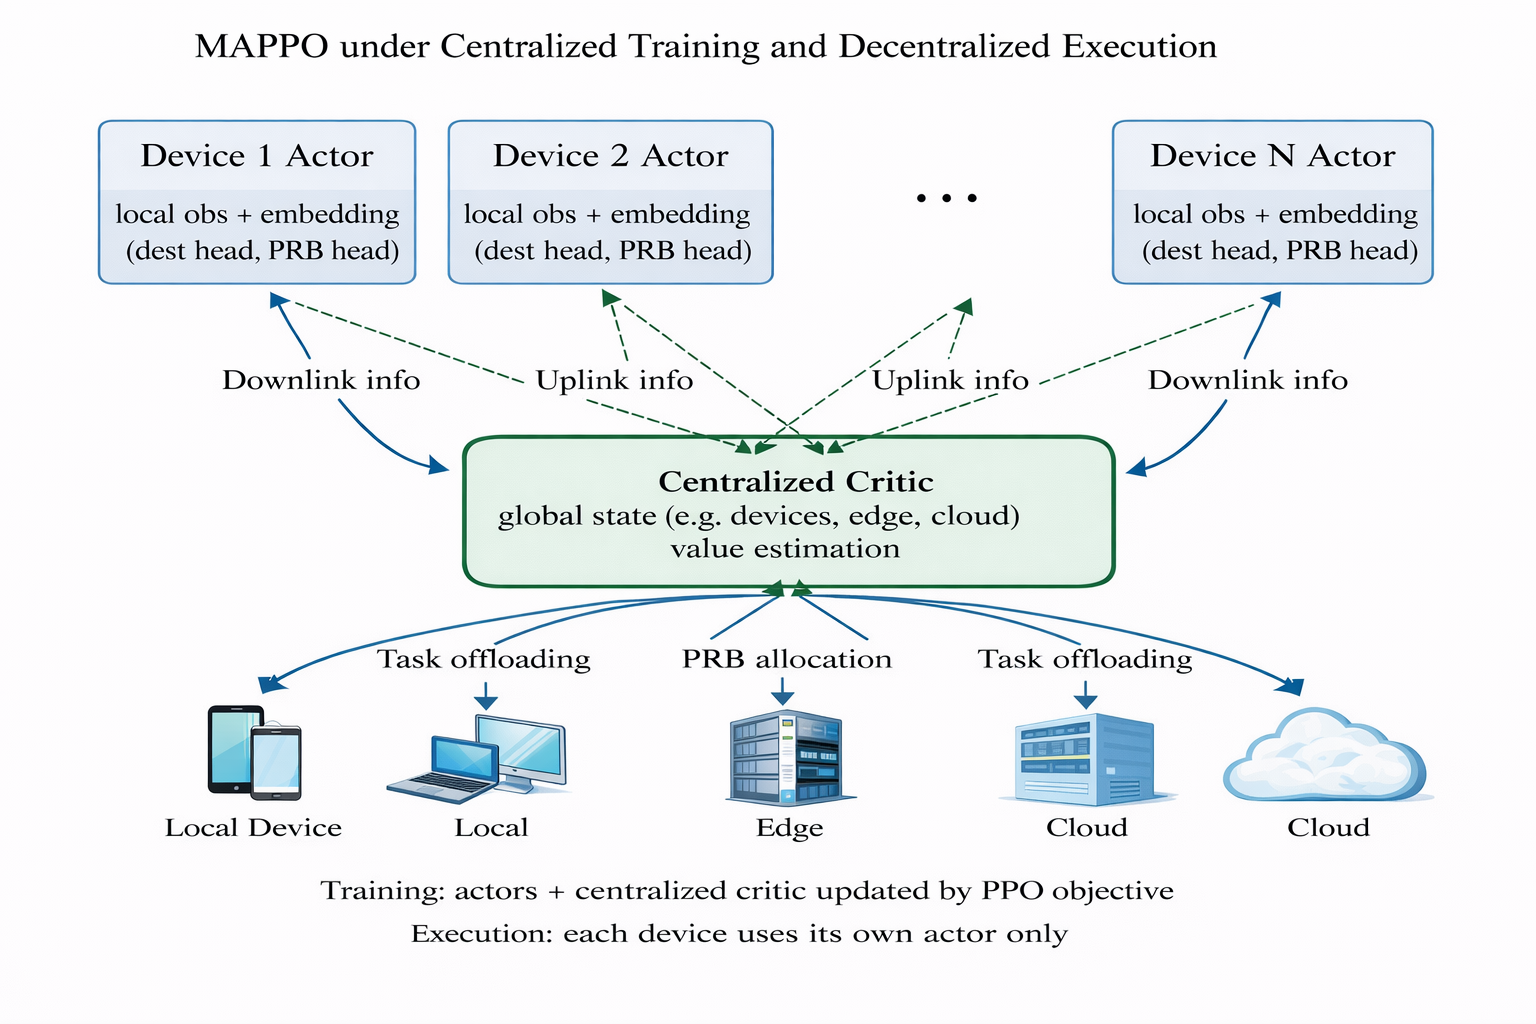
\includegraphics[width=0.92\textwidth]{figures/mappo_ctde_framework.png}
    \caption{Overall MAPPO framework under centralized training and decentralized execution.}
    \label{fig:mappo-ctde-framework}
\end{figure}

Every task-generating device is treated as one agent. When a new task reaches the orchestrator, the corresponding agent receives its observation, selects an execution destination, and, if the task is offloaded, selects a PRB allocation level. The environment then applies the action, executes the task in PureEdgeSim, and returns the resulting reward and transition record to the learner.

\subsection{Observation and State Design}
\label{subsec:observation-state}

The observation design follows the structure implemented in \texttt{DeviceAgentDecisionSupport}. For agent \(i\), the local input is
\begin{align}
o_i = \left(x_i, D_i, m_i\right),
\end{align}
where \(x_i \in \R^{13}\) is the device-level feature vector, \(D_i \in \R^{N_d \times 11}\) is the destination-feature matrix, and \(m_i \in \{0,1\}^{N_d}\) is the destination-feasibility mask.

The 13-dimensional agent feature vector combines normalized task descriptors, source-device resource indicators, and PRB-availability terms. The destination matrix contains one 11-dimensional feature vector for each candidate destination. The candidates are ordered consistently as local execution first, then edge data centers sorted by data-center identifier, and finally cloud destinations. Each destination feature summarizes its load, compute capacity, estimated finish-over-deadline ratio, distance, network admissibility, destination type, and estimated PRB demand.

The global state used by the critic is a 27-dimensional vector,
\begin{align}
s \in \R^{27},
\end{align}
that aggregates system-wide load indicators, PRB usage, task statistics, and tier-level summaries across the local, edge, and cloud layers. In other words, the actor solves a partially observed local decision problem, while the critic evaluates actions against a richer representation of the full environment.

To make the feature design explicit, \Tabref{tab:agent-observation-features} summarizes the 13 local observation dimensions and \Tabref{tab:destination-global-features} summarizes the destination feature matrix together with the additional global-state components.

\begin{table}[htbp]
    \centering
    \begin{tabular}{p{0.18\linewidth}p{0.72\linewidth}}
        \hline
        \textbf{Indices} & \textbf{Meaning} \\
        \hline
        0--4 & Normalized task length, deadline, request size, result size, and container size. \\
        5--8 & Source-device CPU load, source energy level, source running-task count, and best local-VM MIPS. \\
        9--12 & Reachable-edge count, remaining PRB ratio, normalized simulation time, and normalized affordable PRB ceiling. \\
        \hline
    \end{tabular}
    \caption{Agent-observation dimensions implemented in \texttt{DeviceAgentDecisionSupport}.}
    \label{tab:agent-observation-features}
\end{table}

\begin{table}[htbp]
    \centering
    \begin{tabular}{p{0.18\linewidth}p{0.72\linewidth}}
        \hline
        \textbf{Component} & \textbf{Meaning} \\
        \hline
        Destination 0--2 & Destination CPU load, running-task count, and total MIPS. \\
        Destination 3--5 & Estimated finish-over-deadline ratio, normalized distance, and network-admissibility flag. \\
        Destination 6--10 & Local / edge / cloud type flags, VM-count summary, and estimated PRB need. \\
        Global 0--12 & Direct copy of the active agent's 13-dimensional local observation. \\
        Global 13--26 & Source CPU mean/max, source energy mean/max, source running-task mean/max, edge CPU mean/std, edge running-task mean/std, cloud CPU mean, active-task ratio, allocated-PRB ratio, and destination CPU-imbalance std. \\
        \hline
    \end{tabular}
    \caption{Destination-feature groups and global-state composition.}
    \label{tab:destination-global-features}
\end{table}

The destination mask plays a central role in maintaining valid actions. If a destination is out of coverage, lacks a feasible VM, or violates offloading constraints, its mask value is set to zero and the corresponding action logit is suppressed before sampling. This masked policy is more sample efficient than allowing invalid actions and penalizing them afterward.

\subsection{Action Space Design}
\label{subsec:action-space}

The agent action is factorized into a destination head and a PRB head:
\begin{align}
a_i = \left(a_i^{\mathrm{dest}}, a_i^{\mathrm{prb}}\right).
\end{align}
The destination head selects one element from the ordered candidate list. The PRB head selects one out of eight discrete bins. The bins represent relative fractions of the per-task PRB limit:
\begin{align}
\rho \in \{0.02, 0.05, 0.10, 0.20, 0.40, 0.60, 0.80, 1.00\}.
\end{align}
Given the simulator setting \(\texttt{maxPerTask}=50\), the selected ratio is converted into an integer reservation capped at 50 blocks.

If the chosen destination is local execution, the PRB action is ignored and replaced by zero because no wireless upload is required. In the implementation, the PRB log-probability and entropy contributions are also neutralized for such local actions so that the policy is not penalized for an irrelevant bandwidth choice.

Although destination masking prevents most invalid actions, a final destination fallback rule is retained for robustness. If the sampled action still points to an infeasible destination at execution time, the system falls back to the feasible destination with the shortest estimated completion time. In the final MAPPO evaluation runs used in this report, the fallback count is zero across all three seeds, indicating that the trained policy learns to stay within the valid action region.

\subsection{Network Architecture}
\label{subsec:network-architecture}

\subsubsection{TurnActor (MAPPO Actor)}

The MAPPO actor is implemented as a \texttt{TurnActor}. Each agent identifier is mapped to a learnable 16-dimensional embedding \(e_i\). The embedding is concatenated with the 13-dimensional agent observation and passed through a two-layer multilayer perceptron with hidden size 128 and \(\tanh\) activations:
\begin{align}
h_i = f_{\theta}^{\mathrm{agent}}\left([x_i ; e_i]\right).
\end{align}
The embedding table can be resized dynamically when the number of task-generating devices changes, which avoids hard-coding the agent count into the model definition.

Each candidate destination feature vector \(d_{i,j}\) is concatenated with the repeated agent hidden state and encoded by a destination-specific multilayer perceptron:
\begin{align}
u_{i,j} = f_{\theta}^{\mathrm{dest}}([d_{i,j}; h_i]),
\end{align}
again using a two-layer MLP with hidden size 128 and \(\tanh\) activations. A linear destination head then scores every encoded candidate:
\begin{align}
\ell_{i,j}^{\mathrm{dest}} = w_{\mathrm{dest}}^\top u_{i,j} + b_{\mathrm{dest}},
\end{align}
followed by masked softmax and categorical sampling:
\begin{align}
\pi_{\theta}^{\mathrm{dest}}(j \mid o_i) =
\mathrm{Softmax}\!\left(\mathrm{Mask}\!\left(\ell_{i,j}^{\mathrm{dest}}, m_i\right)\right).
\end{align}

The PRB head is conditioned on the selected destination. In the implementation, the hidden vector of the selected destination is concatenated with the agent hidden state and passed to a dedicated PRB head:
\begin{align}
\ell_i^{\mathrm{prb}} = g_{\theta}\left([h_i ; u_{i,a_i^{\mathrm{dest}}}]\right),
\end{align}
followed by
\begin{align}
\pi_{\theta}^{\mathrm{prb}}(k \mid o_i, a_i^{\mathrm{dest}}) =
\mathrm{Softmax}\!\left(\ell_i^{\mathrm{prb}}\right).
\end{align}
This coupling is important because the desirable PRB level differs substantially between nearby edge nodes and the farther cloud tier. In code, the PRB head is realized as \texttt{Linear(256,128)} \(\rightarrow\) \(\tanh\) \(\rightarrow\) \texttt{Linear(128,8)}.

\subsubsection{CentralCritic}

The centralized critic takes the 27-dimensional global state as input and outputs one scalar value estimate:
\begin{align}
V_{\phi}(s) = f_{\phi}^{\mathrm{critic}}(s).
\end{align}
The critic uses a two-layer MLP with hidden size 256 and \(\tanh\) activations. Because the critic sees aggregated system information that is unavailable to an individual device, it can provide a more stable baseline for policy optimization than a purely local value function.

\subsubsection{PPO Baseline Actor}

The PPO baseline shares the same destination encoder, PRB head, and overall dual-head logic, but removes the learnable agent embedding. Its actor receives only the raw 13-dimensional device observation before constructing the same destination-conditioned hidden states. As a result, PPO must represent all device roles through a single shared feature space, whereas MAPPO can condition each policy evaluation on an explicit agent identity. This architectural difference is the main controlled distinction between the two RL methods.

\subsection{Reward Function Design}
\label{subsec:reward-function}

The reward is defined at the task level:
\begin{align}
R =
\begin{cases}
-5.0, & \text{if the task fails}, \\
5.0 - 2.0 \cdot latencyRatio - 0.5 \cdot energyNorm - 1.0 \cdot networkCost,
& \text{if the task succeeds}.
\end{cases}
\label{eq:reward}
\end{align}
Here,
\begin{align}
latencyRatio &= \frac{\text{actual latency}}{\text{maximum allowed latency}}, \\
energyNorm &= \text{P95-normalized transmission energy}, \\
networkCost &= \frac{\text{reserved PRB blocks}}{50}.
\end{align}

This formulation explicitly favors deadline satisfaction while still discouraging wasteful wireless reservations and excessive transmission energy. A failed task receives a fixed negative reward because lateness, mobility loss, or network failure all indicate a clear scheduling breakdown. For successful tasks, the positive base reward is gradually reduced according to delay, energy, and PRB cost. The weighting prioritizes latency first, then energy, then wireless occupancy.

\subsection{Training Algorithm}
\label{subsec:training-algorithm}

Policy optimization follows the clipped PPO objective \cite{schulman2017ppo}. For trajectory sample \(t\),
\begin{align}
L^{\mathrm{clip}}(\theta) =
\E_t \left[
\min \left(
r_t(\theta)\hat{A}_t,\,
\mathrm{clip}(r_t(\theta), 1-\epsilon, 1+\epsilon)\hat{A}_t
\right)
\right],
\end{align}
where
\begin{align}
r_t(\theta) =
\frac{\pi_{\theta}(a_t \mid o_t)}{\pi_{\theta_{\mathrm{old}}}(a_t \mid o_t)}.
\end{align}

For the finalized training artifact used in this report, the implementation adopts a one-step event-level advantage rather than a long-horizon bootstrapped estimator. Specifically, the update code uses
\begin{align}
R_t &= r_t, \\
\hat{A}_t &= r_t - V_{\phi}(s_t),
\end{align}
followed by minibatch normalization of \(\hat{A}_t\). This choice matches the event-driven nature of the environment: each transition already corresponds to a largely self-contained offloading transaction whose reward summarizes latency, energy, and PRB usage after the task outcome is known. The shared Python utilities still contain a generic GAE helper for future extensions, but the MAPPO and PPO runs reported here use the immediate-return form above.

Entropy regularization is linearly annealed from 0.02 to 0.002, encouraging exploration early in training and sharper decisions later. The main hyperparameters are listed in \Tabref{tab:training-hyperparameters}.

\begin{table}[htbp]
    \centering
    \begin{tabular}{p{0.48\linewidth}p{0.28\linewidth}}
        \hline
        \textbf{Hyperparameter} & \textbf{Value} \\
        \hline
        Training episodes & 40 \\
        PPO clip \(\epsilon\) & 0.1 \\
        Actor learning rate & \(3 \times 10^{-4}\) \\
        Critic learning rate & \(3 \times 10^{-4}\) \\
        PPO epochs per update & 4 \\
        Minibatch size & 1024 \\
        Episodes per update & 1 \\
        Entropy coefficient & 0.02 \(\rightarrow\) 0.002 \\
        Max gradient norm & 0.5 \\
        Agent embedding dimension & 16 \\
        Actor hidden dimension & 128 \\
        Critic hidden dimension & 256 \\
        PRB bins & 8 \\
        \hline
    \end{tabular}
    \caption{Main training hyperparameters used for MAPPO and the PPO baseline.}
    \label{tab:training-hyperparameters}
\end{table}

The runtime configuration still records a nominal \(\gamma = 0.99\) for compatibility with the shared training scripts, but the reported runs do not bootstrap across future rewards in the update rule above.

Algorithmically, one training episode proceeds as follows.
\begin{enumerate}
    \item Java starts a 30-minute PureEdgeSim episode and exposes the MARL interface through \texttt{RLEnvServer}.
    \item Every time a task reaches the orchestrator, the active device sends a masked local observation to Python.
    \item Python samples a destination and PRB action, sends the decision back, and stores the resulting transition.
    \item At the end of the episode, the centralized critic computes values, advantages are estimated, and PPO updates the actor and critic for four epochs.
    \item The best-performing checkpoints are then reused for offline inference and multi-seed evaluation.
\end{enumerate}

The resulting method preserves decentralized execution at deployment time while still exploiting centralized information during training, which is the key reason MAPPO is attractive for large, interacting edge-computing systems.
